\documentclass[aspectratio=169]{beamer}
\usepackage[utf8]{inputenc}
\usepackage{bookman}
\usetheme{Dresden}
\usepackage{graphicx}
\usepackage{hyperref}
\usepackage{todonotes}
\usepackage{xcolor}
\definecolor{LightGray}{gray}{0.9}
\usepackage{minted}
\usemintedstyle{manni}
\setminted{fontsize=\scriptsize,
           bgcolor=LightGray,
           breaklines,
           gobble=4
}

\title[Electronic Design Automation]{Electronics Design Automation: Schematic Capture \& PCB Layout}
\author{MedTech Prototyping Skills (BME290L)}
\institute[Palmeri (BME290L)]{Mark L. Palmeri, M.D., Ph.D.}
\date{Fall 2023}
\logo{
\includegraphics[width=0.1\textwidth]{BME-HorizontalLogo-Web-Blue.png}}

\begin{document}

\frame{\titlepage}

\section{Overview}

\frame{
    \begin{center}
        
\includegraphics[width=0.15\textwidth]{kicad_logo_small.png}
    \end{center}

    \begin{itemize}
        \item Installation: \url{https://kicad.org}
        \begin{itemize}
          \item Certain video cards will not work well with the PCB tool.  In that case, disable the \textit{Accelerated} toolset and choose the \textit{Fallback} graphics toolset.
          \item On Macs, your part / footprint / model libraries might not be detected automatically after installation.  You might need to manually point Kicad at them in a path similar to: \texttt{Macintosh/Library/Application Support/kicad/templates/sym-lib-table/}.
        \end{itemize}
        \item Documentation: \url{https://docs.kicad.org/6.0/en/getting_started_in_kicad/getting_started_in_kicad.html}
    \end{itemize}
}

\section{Schematics}

\frame{
  \frametitle{UI/UX}

  \centerline{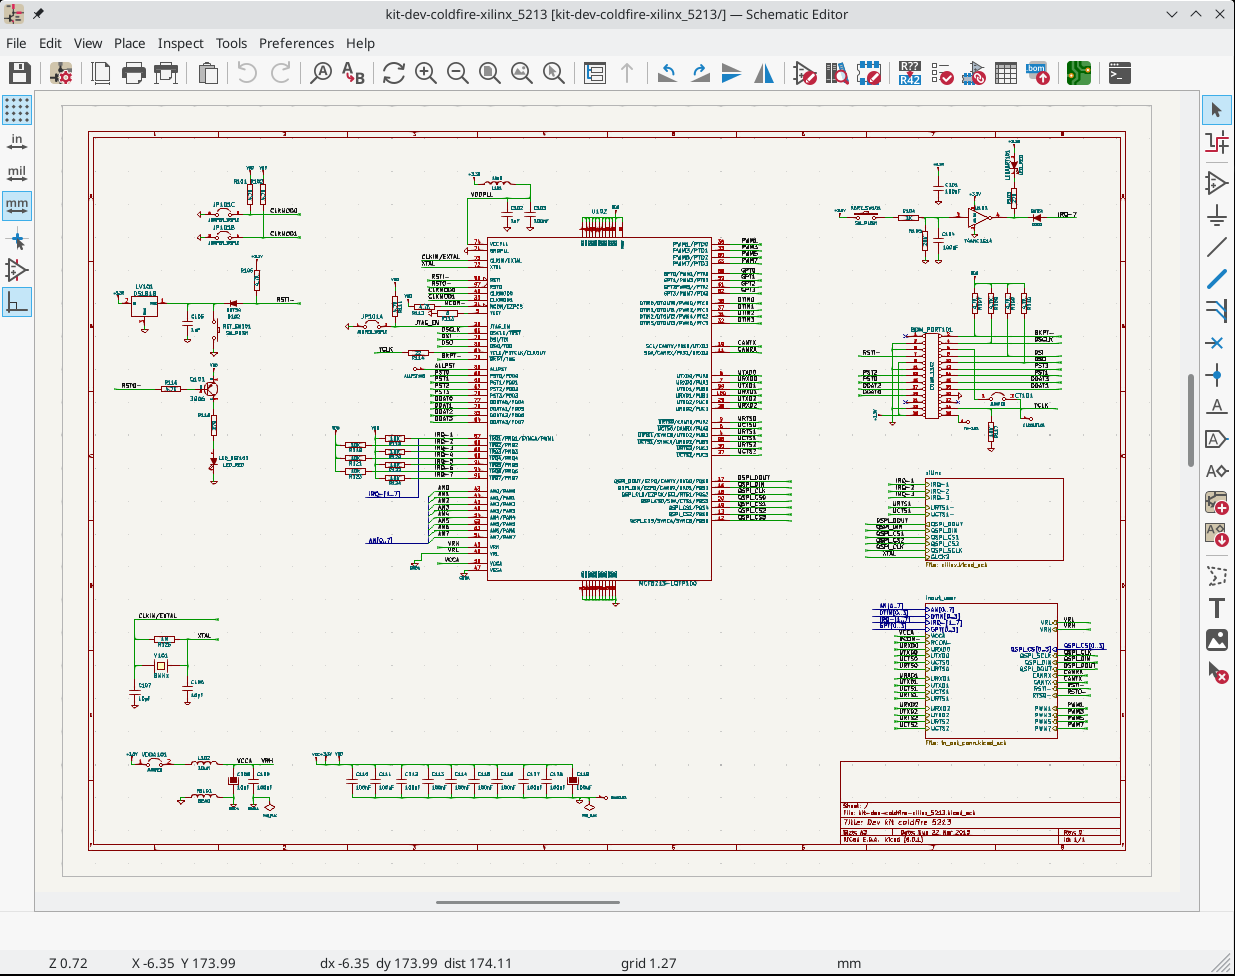
\includegraphics[width=0.5\textwidth]{commands_overview.png}}

  \begin{center}
    \begin{footnotesize}
      \url{https://docs.kicad.org/6.0/en/eeschema/eeschema.html\#schematic-editing-operations}
    \end{footnotesize}
  \end{center}
}

\frame{
  \frametitle{Schematic Capture}
  \begin{columns}
  \begin{column}{0.7\textwidth}
    \begin{enumerate}
      \item Create a New Project, which creates a schematic file.
      \item \textbf{DO NOT CHANGE THE GRID SPACING!!}
      \item Setup \texttt{Page Settings...}, using \href{https://semver.org/}{semantic versioning} for ``Revision''.
      \item Configure \texttt{Schematic Setup...}, including \texttt{Project:Net Classes}.
    \end{enumerate}
  \end{column}
  \begin{column}{0.3\textwidth}
    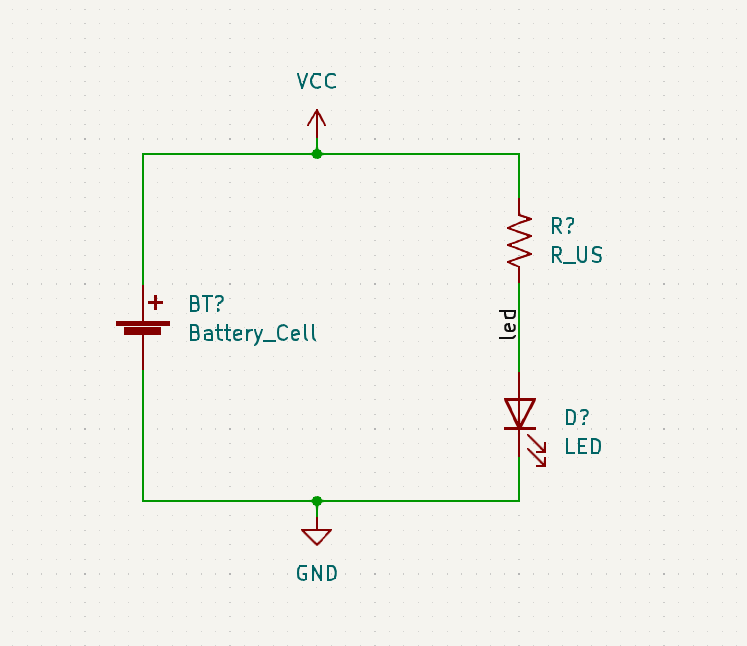
\includegraphics[width=1.0\textwidth]{symbols-labeled.png}
  \end{column}
  \end{columns}
}
	  
\begin{frame}
   \begin{columns}
    \begin{column}{0.6\textwidth}
      \begin{enumerate}
        \setcounter{enumi}{4}
        \item Place component / part (\texttt{Place Symbol}) using default library.
        If component doesn't exist, then you either need to:
        \begin{itemize}
          \item Download the part from an online database (e.g., \href{https://www.snapeda.com/}{SnapEDA})
          \item Create part using the \texttt{Library Editor}.
        \end{itemize}
        \item Annotate components (give each component a unique label)
        \item Assign component values
        \item Label nets with meaningful names
        \begin{itemize}
            \item Nets are like nodes; common voltage connections.
            \item Use Global net labels to avoid connection chaos.
        \end{itemize}
      \end{enumerate}
    \end{column}
    \begin{column}{0.4\textwidth}
      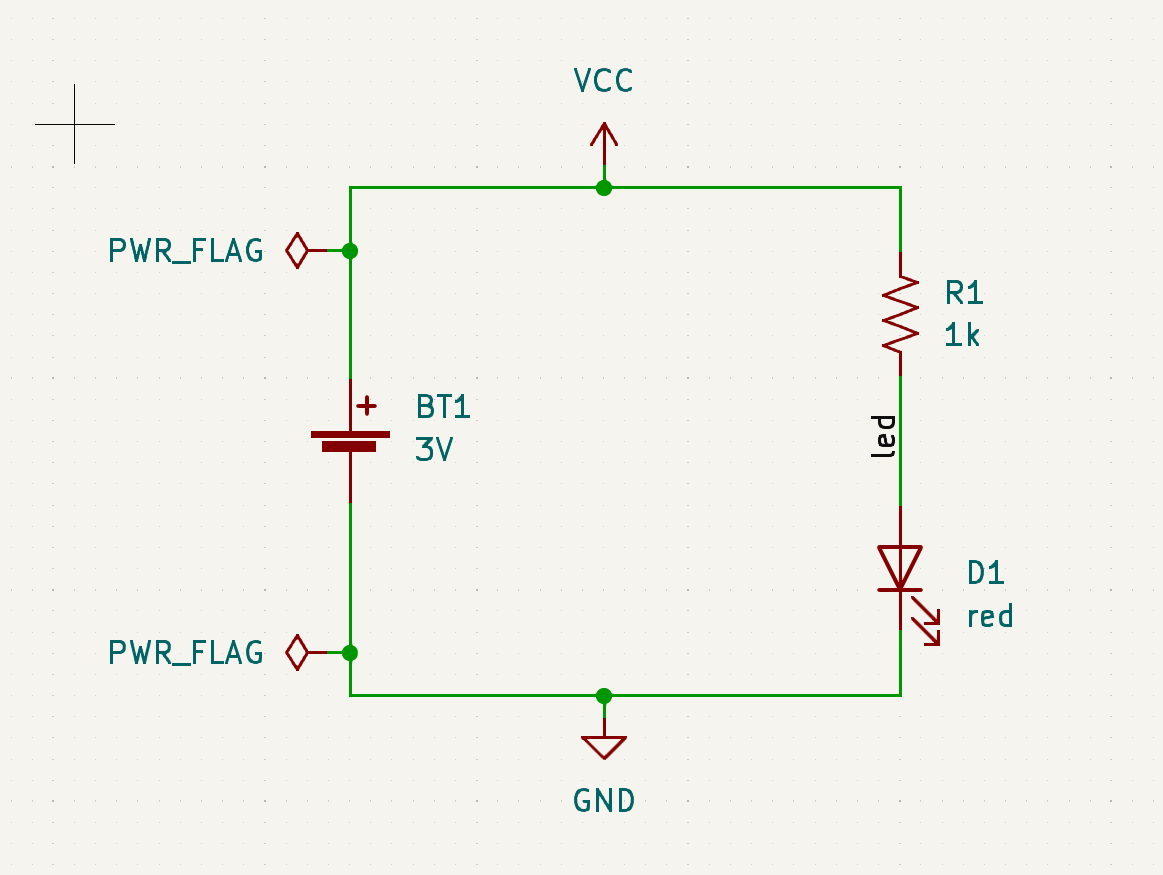
\includegraphics[width=1.0\textwidth]{symbols-pwr-flag.png}   
    \end{column}
   \end{columns}
\end{frame}

\section{Power}
\begin{frame}
  \frametitle{Power Ports}

  \begin{columns}
    \begin{column}{0.6\textwidth}
      \begin{itemize}
        \item Power ports, including ground references, are also global net labels.
        \item Component pins can be explicitly designated power in/out (in contrast to signal).
        \item Power, ideally, cascades top-to-bottom (\texttt{+} $\rightarrow$
        \texttt{GND} [$\rightarrow$ \texttt{-}]) on the schematic.
      \end{itemize}
    \end{column}
    \begin{column}{0.4\textwidth}
      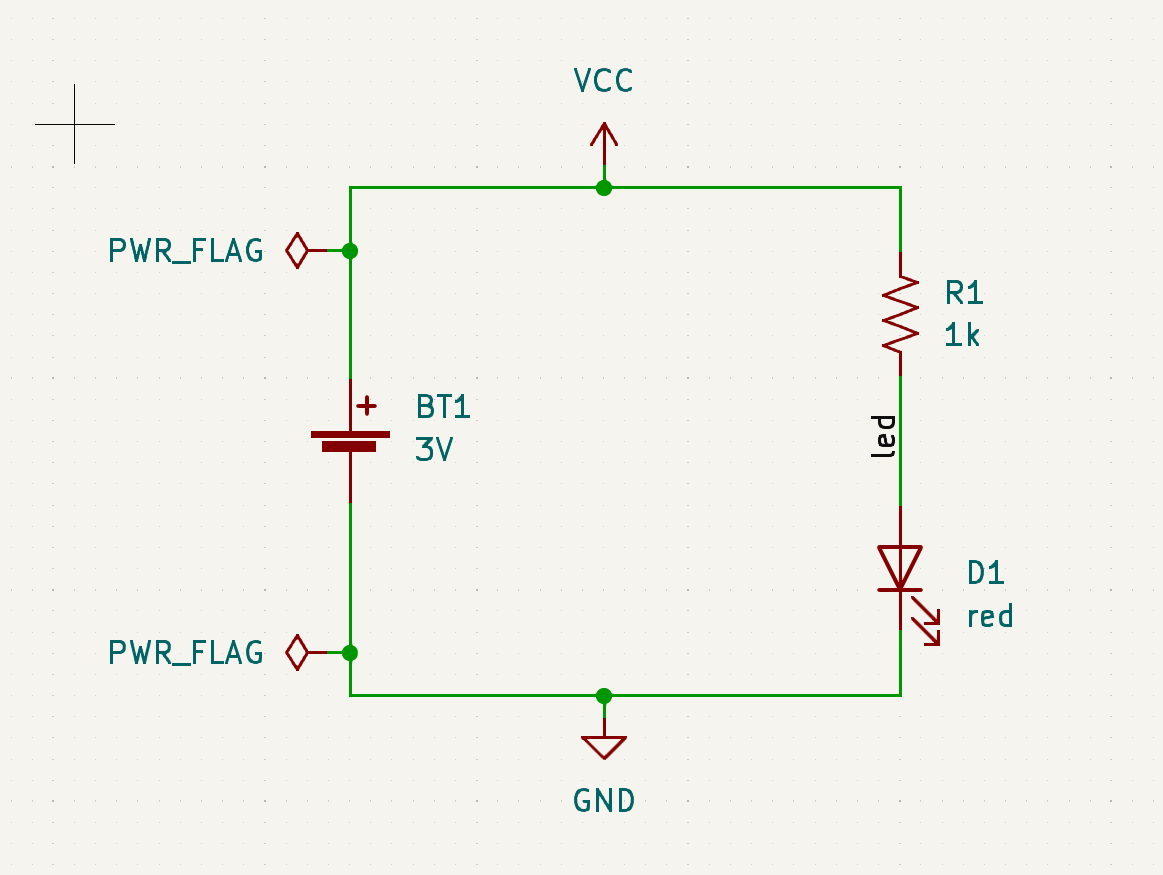
\includegraphics[width=1.0\textwidth]{symbols-pwr-flag.png}   
    \end{column}
\end{columns}
\end{frame}

\section{ERC}
\begin{frame}
  \frametitle{Electrical Rules Check (ERC)}
  \begin{columns}
    \begin{column}{0.6\textwidth}
      \begin{itemize}
        \item Check the validity of the schematic
        \item Common error: ``Input Power pin not driven by any Output Power pins''
        \begin{itemize}
          \item KiCad checks to make sure that power can ``drive'' components that demand that input.
          \item You can explicitly indicate this in the schematic using the
          \texttt{PWR\_FLAG} symbol attached to the net in question.
          \item Might need to re-map pin types (\texttt{Properties:Edit Symbol:Pin Table}).
        \end{itemize}
      \end{itemize}
    \end{column}
    \begin{column}{0.4\textwidth}
      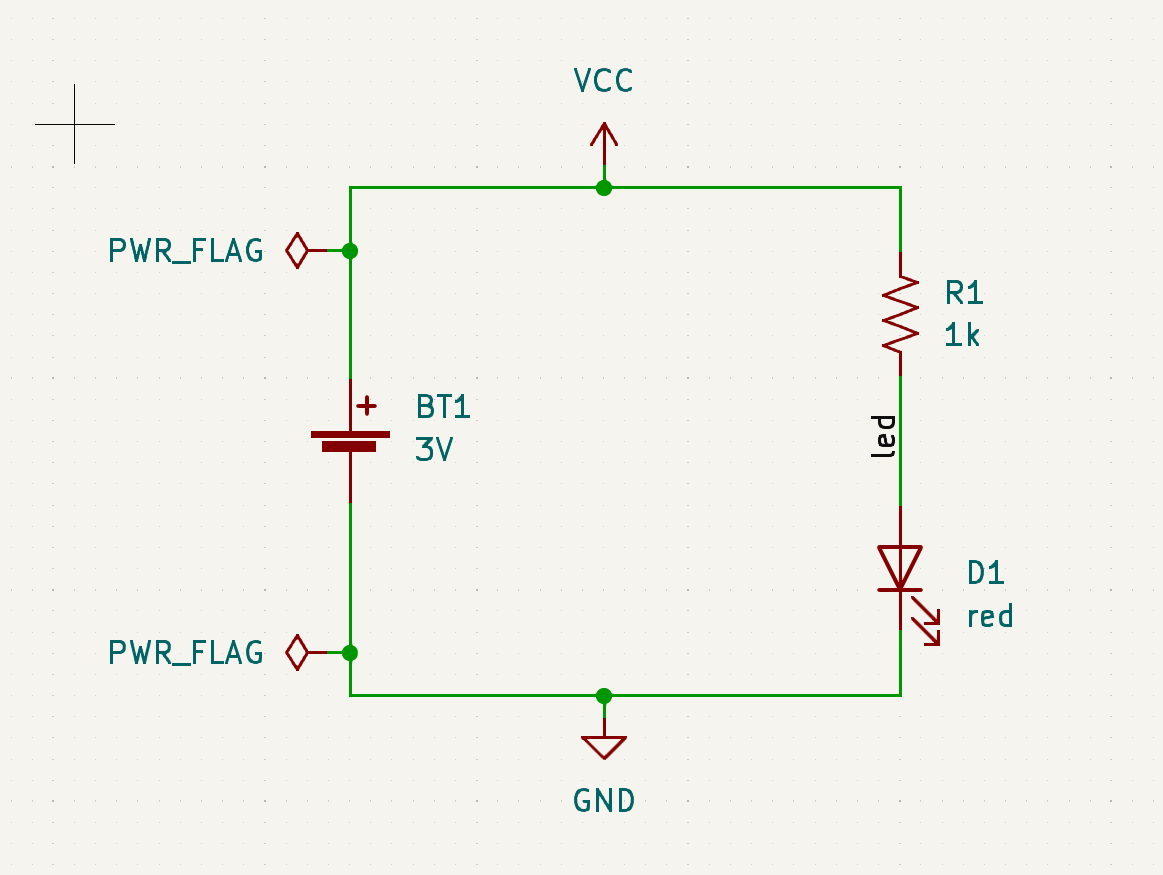
\includegraphics[width=1.0\textwidth]{symbols-pwr-flag.png}   
    \end{column}
  \end{columns}
\end{frame}

\section{Best Practices}
\frame{
   \frametitle{Best Practices}
   \begin{itemize}
      \item Signal, ideally, flows left-to-right (input $\rightarrow$ output).
      \item Outline and label functional blocks.  Use \texttt{Heirarchical
      Sheets} to organize more clearly-defined sub-circuits.
      \item Can include non-electrical items, like \texttt{Mounting Holes}.
      \item Add Test Pins/Pads to nets you will want to verify during testing.
      \begin{itemize}
        \item Power nets
        \item Signal I/O
      \end{itemize}
      \item Use \texttt{No-Connection} flags for pins that are intentionally
       not connected to other components.
      \item You can create a Bill of Materials (BOM) based on your schematic.
   \end{itemize}
 }

 \begin{frame}
  \centerline{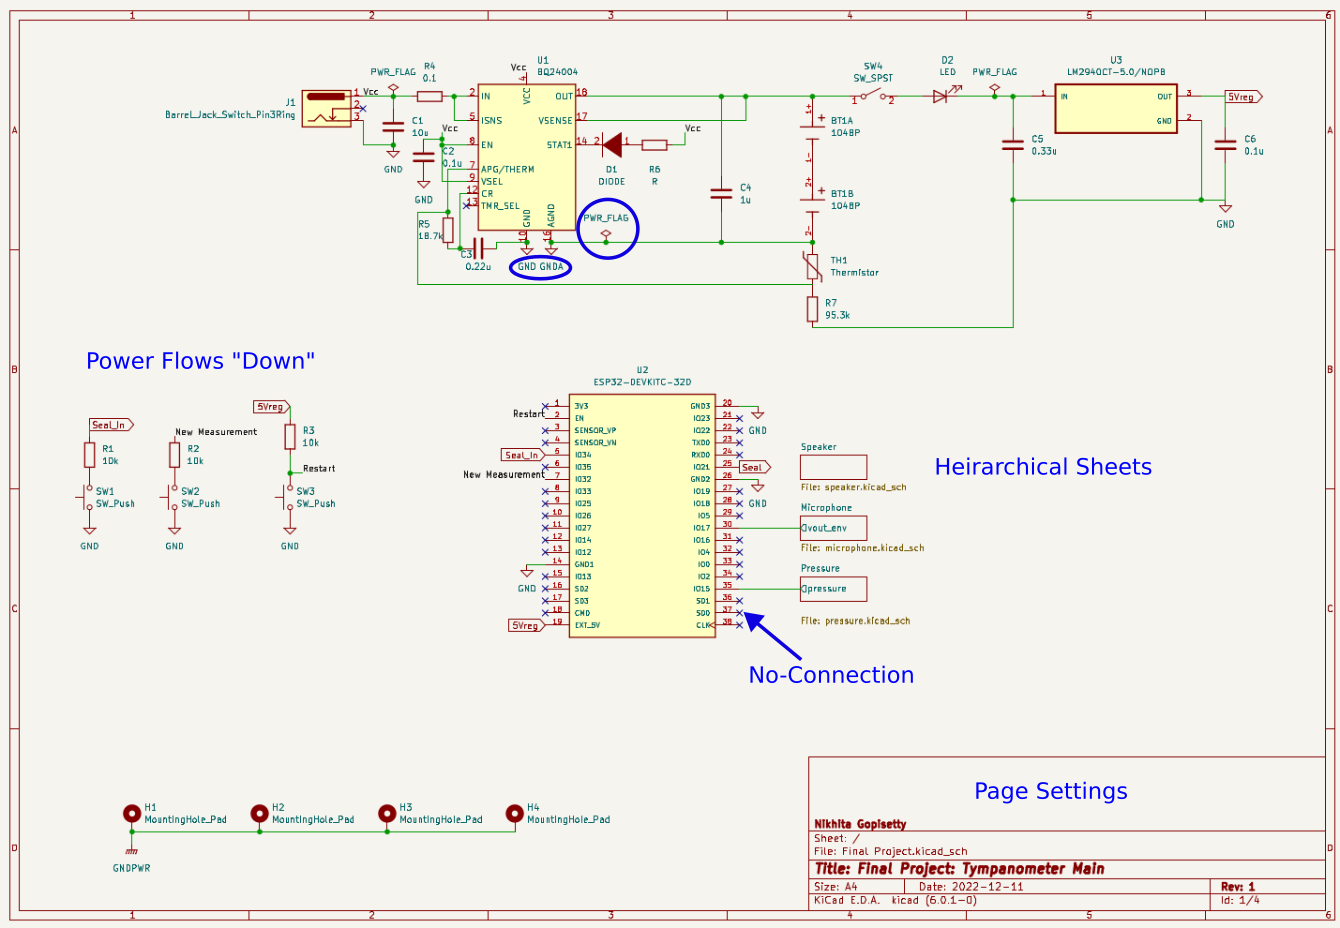
\includegraphics[width=0.7\textwidth]{schematic_annotated.png}}
 \end{frame}

\section{In-class Exercise}

\begin{frame}
  \frametitle{A current project...}

  \centerline{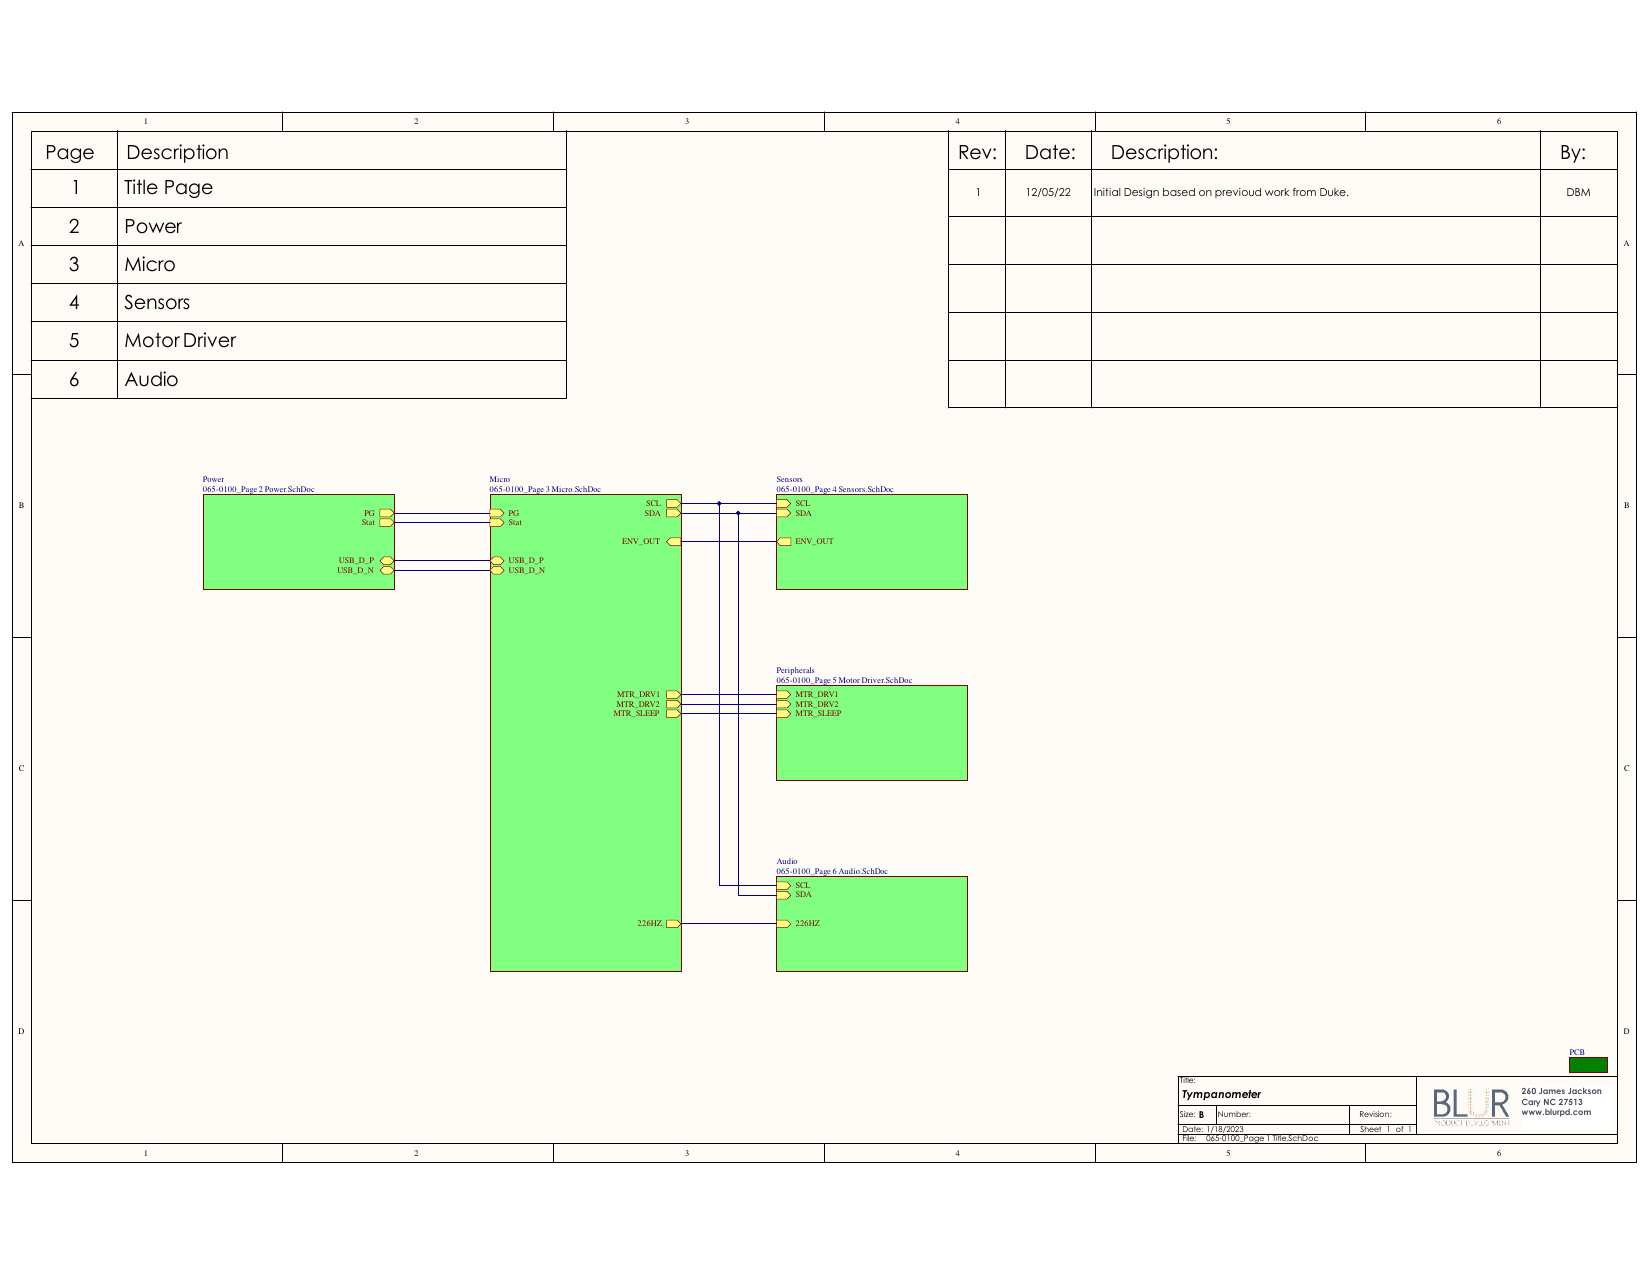
\includegraphics[width=0.6\textwidth]{065-0100_Main_Board-1.png}}
\end{frame}

\begin{frame}
  \frametitle{A current project...}

  \centerline{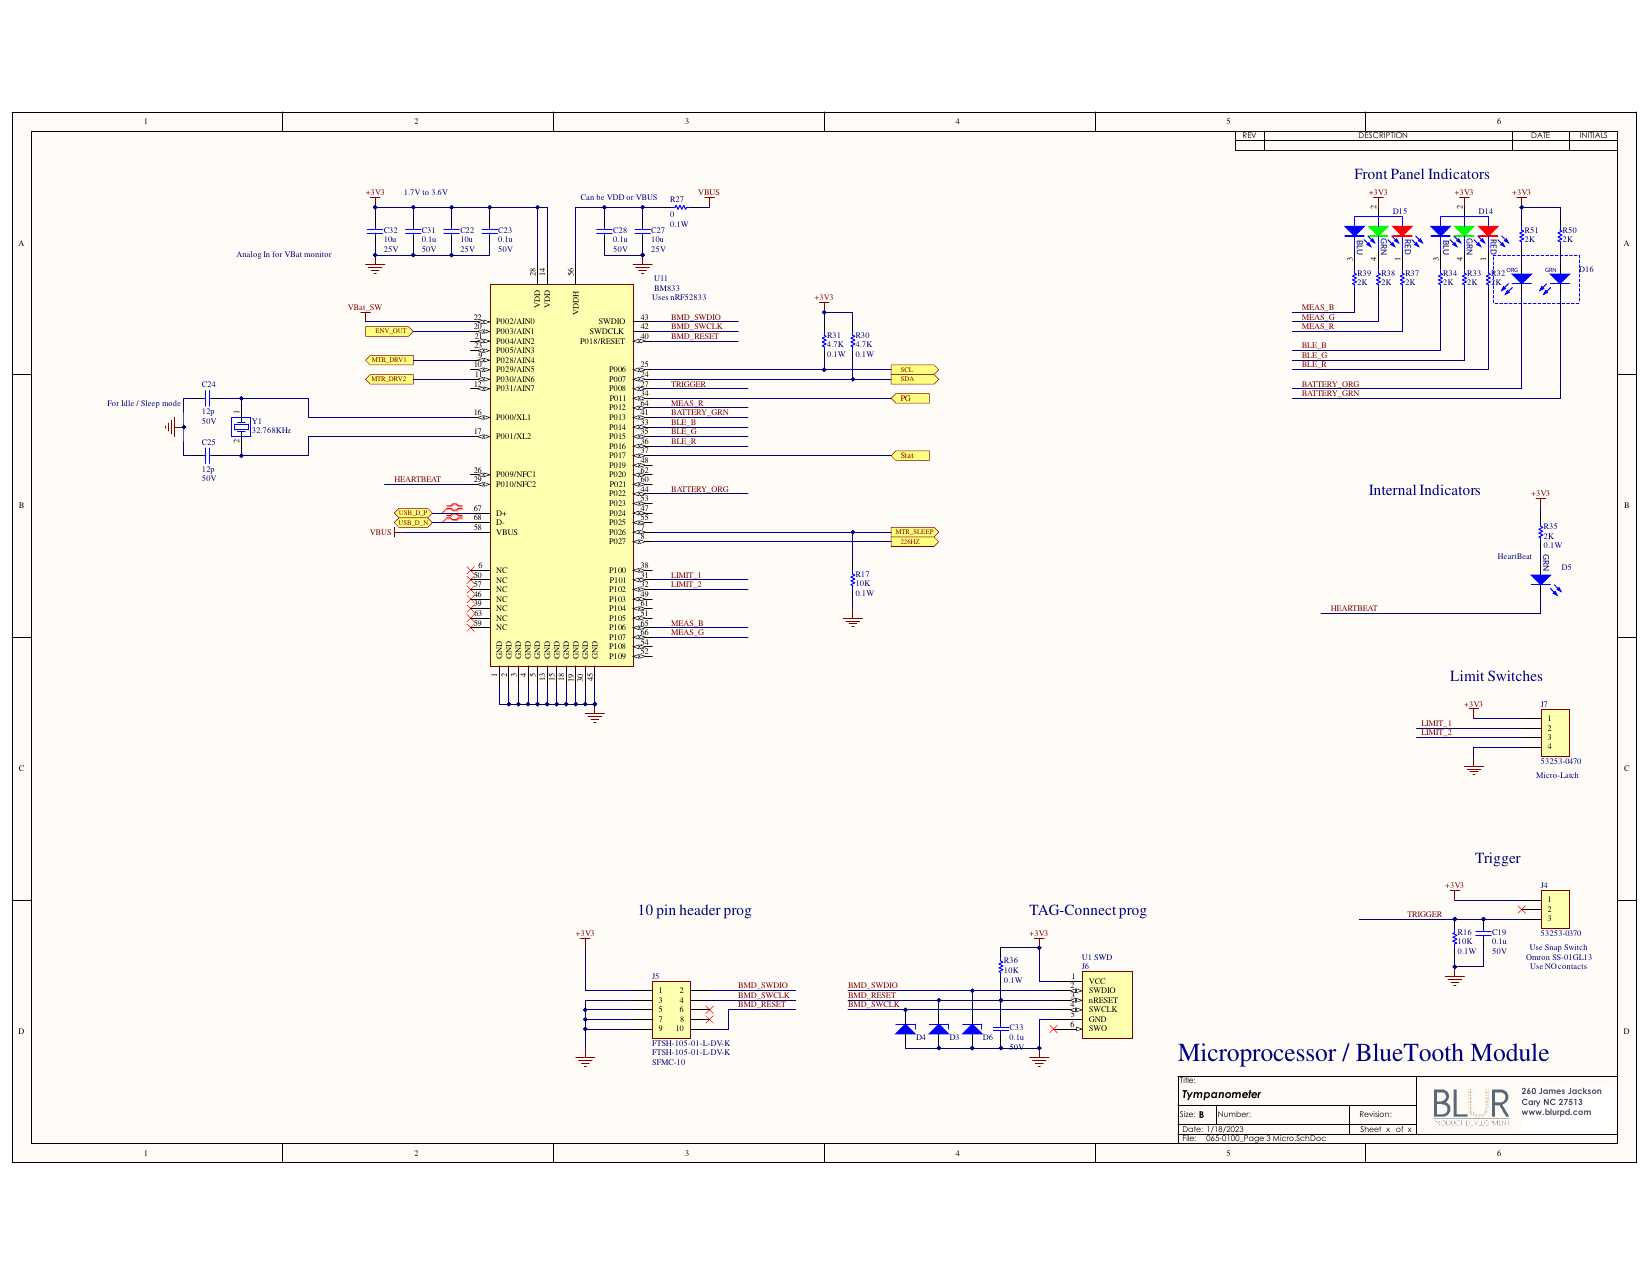
\includegraphics[width=0.6\textwidth]{065-0100_Main_Board-5.png}}
\end{frame}

\begin{frame}
  \frametitle{A current project...}

  \centerline{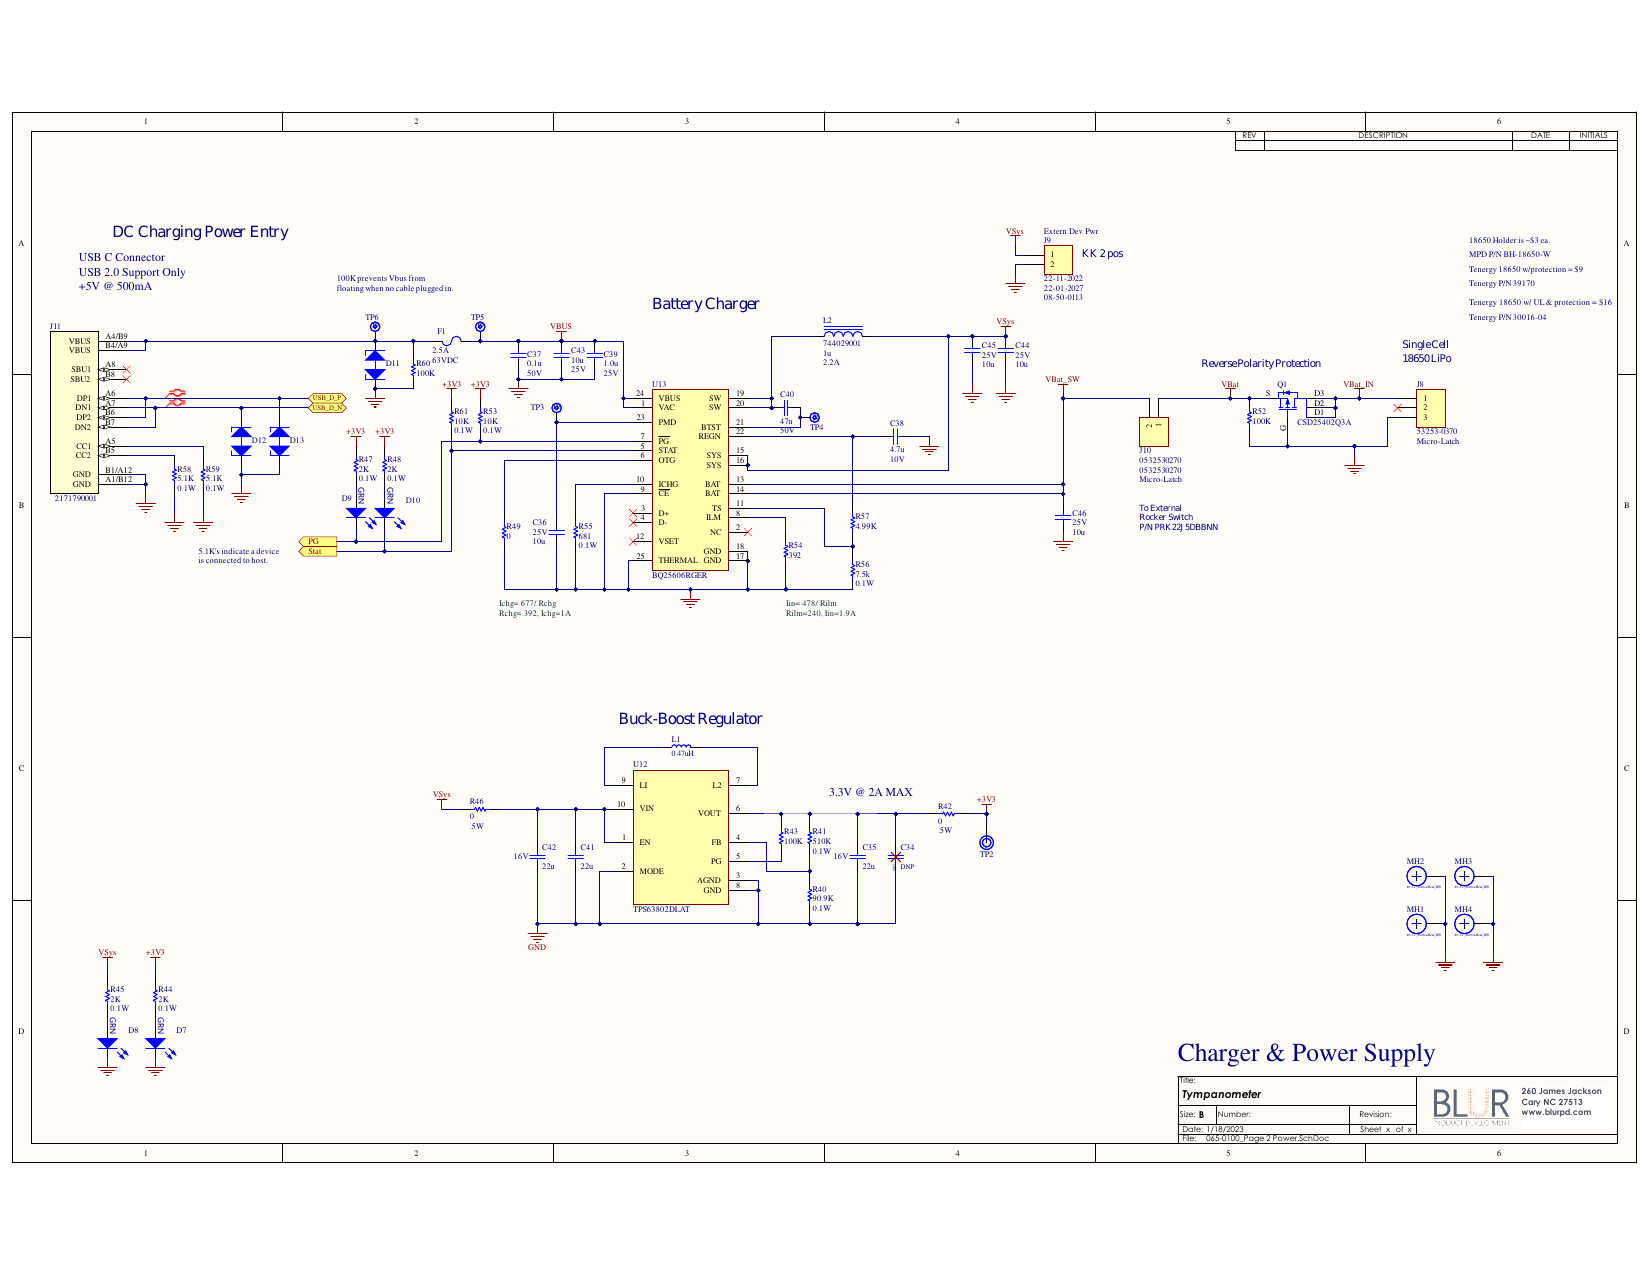
\includegraphics[width=0.6\textwidth]{065-0100_Main_Board-6.png}}
\end{frame}

\begin{frame}
  \frametitle{A current project...}

  \centerline{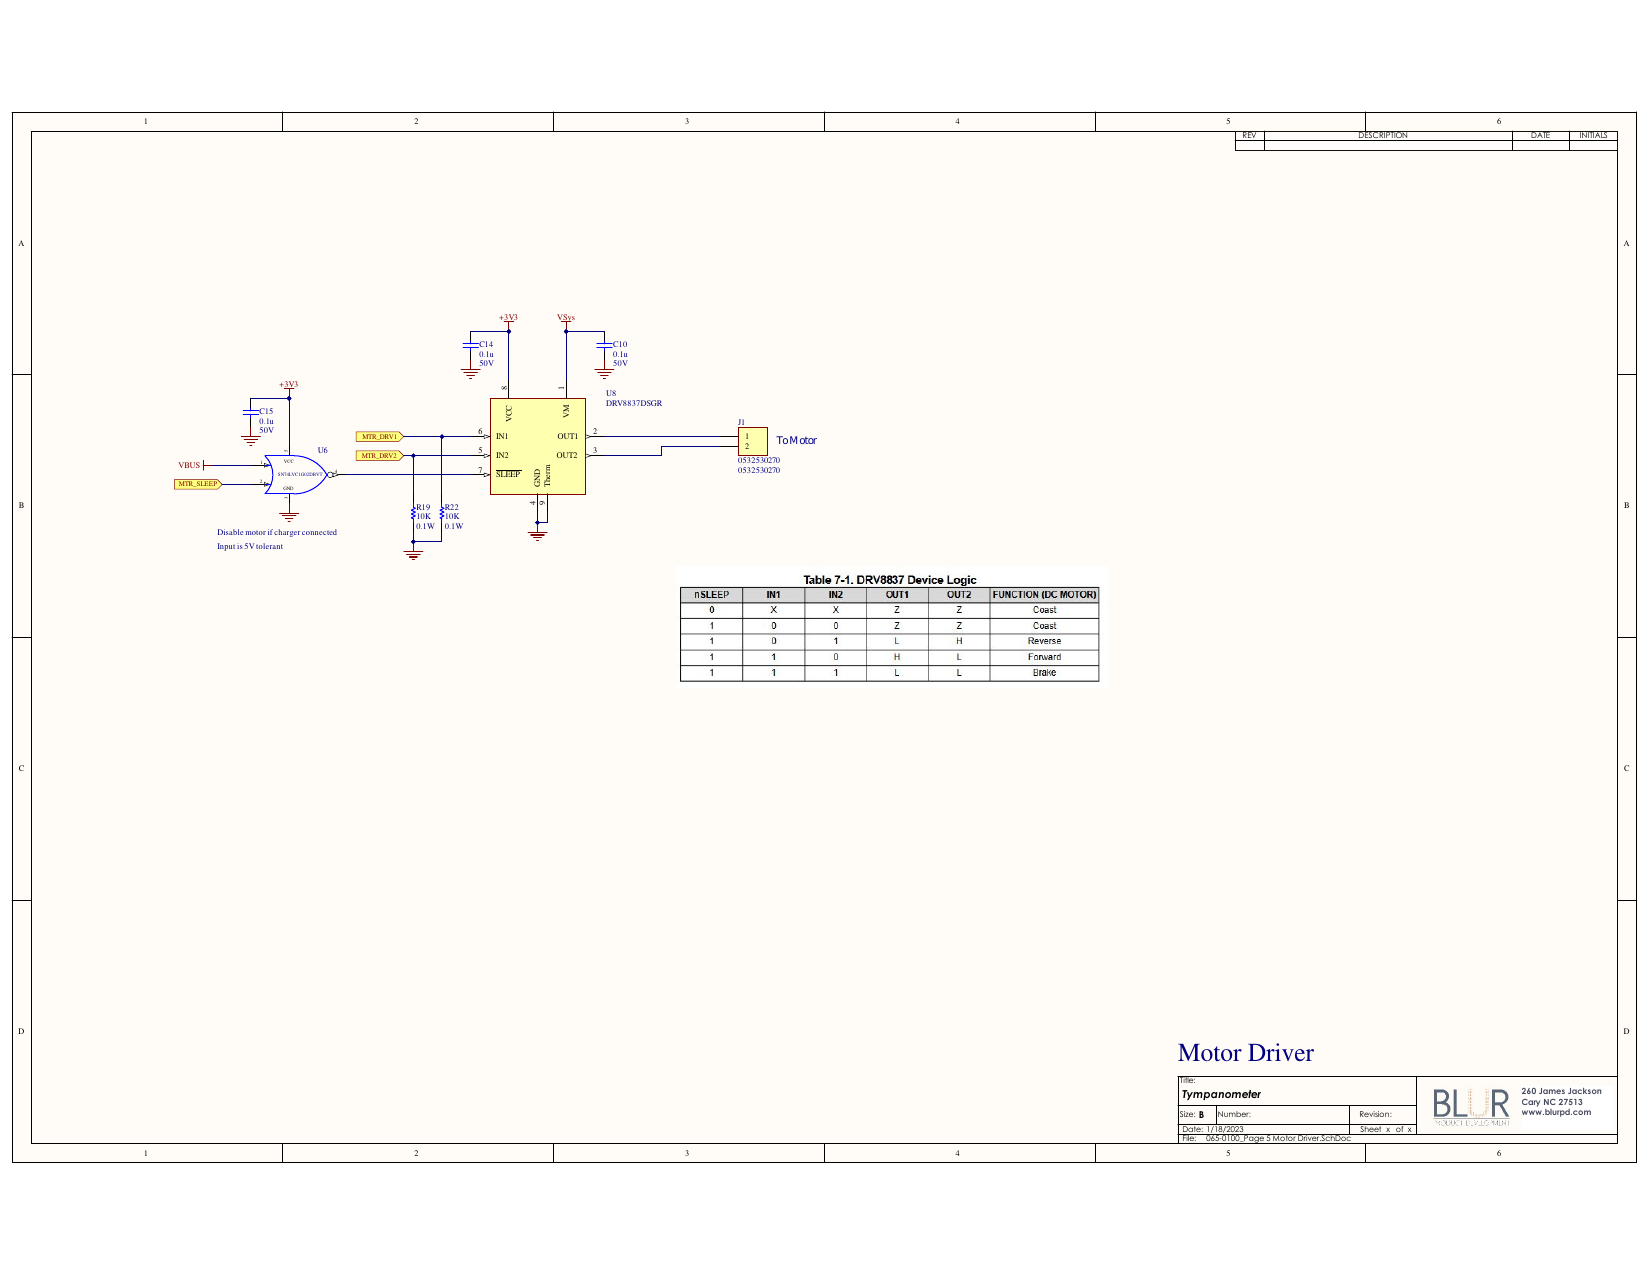
\includegraphics[width=0.6\textwidth]{065-0100_Main_Board-3.png}}
\end{frame}

\section{PCB Layout}

\begin{frame}
    \frametitle{Why a PCB?}
  
    \begin{columns}
      \begin{column}{0.5\textwidth}
        \begin{itemize}
          \item Breadboards are good for simple testing, but not robust.
          \item Need to reduce form factor.
          \item Reduce noise, capacitive effects, etc.
          \item SMD (versus thru-hole) components are becoming ubiquitous.
        \end{itemize}
      \end{column}
      \begin{column}{0.5\textwidth}
        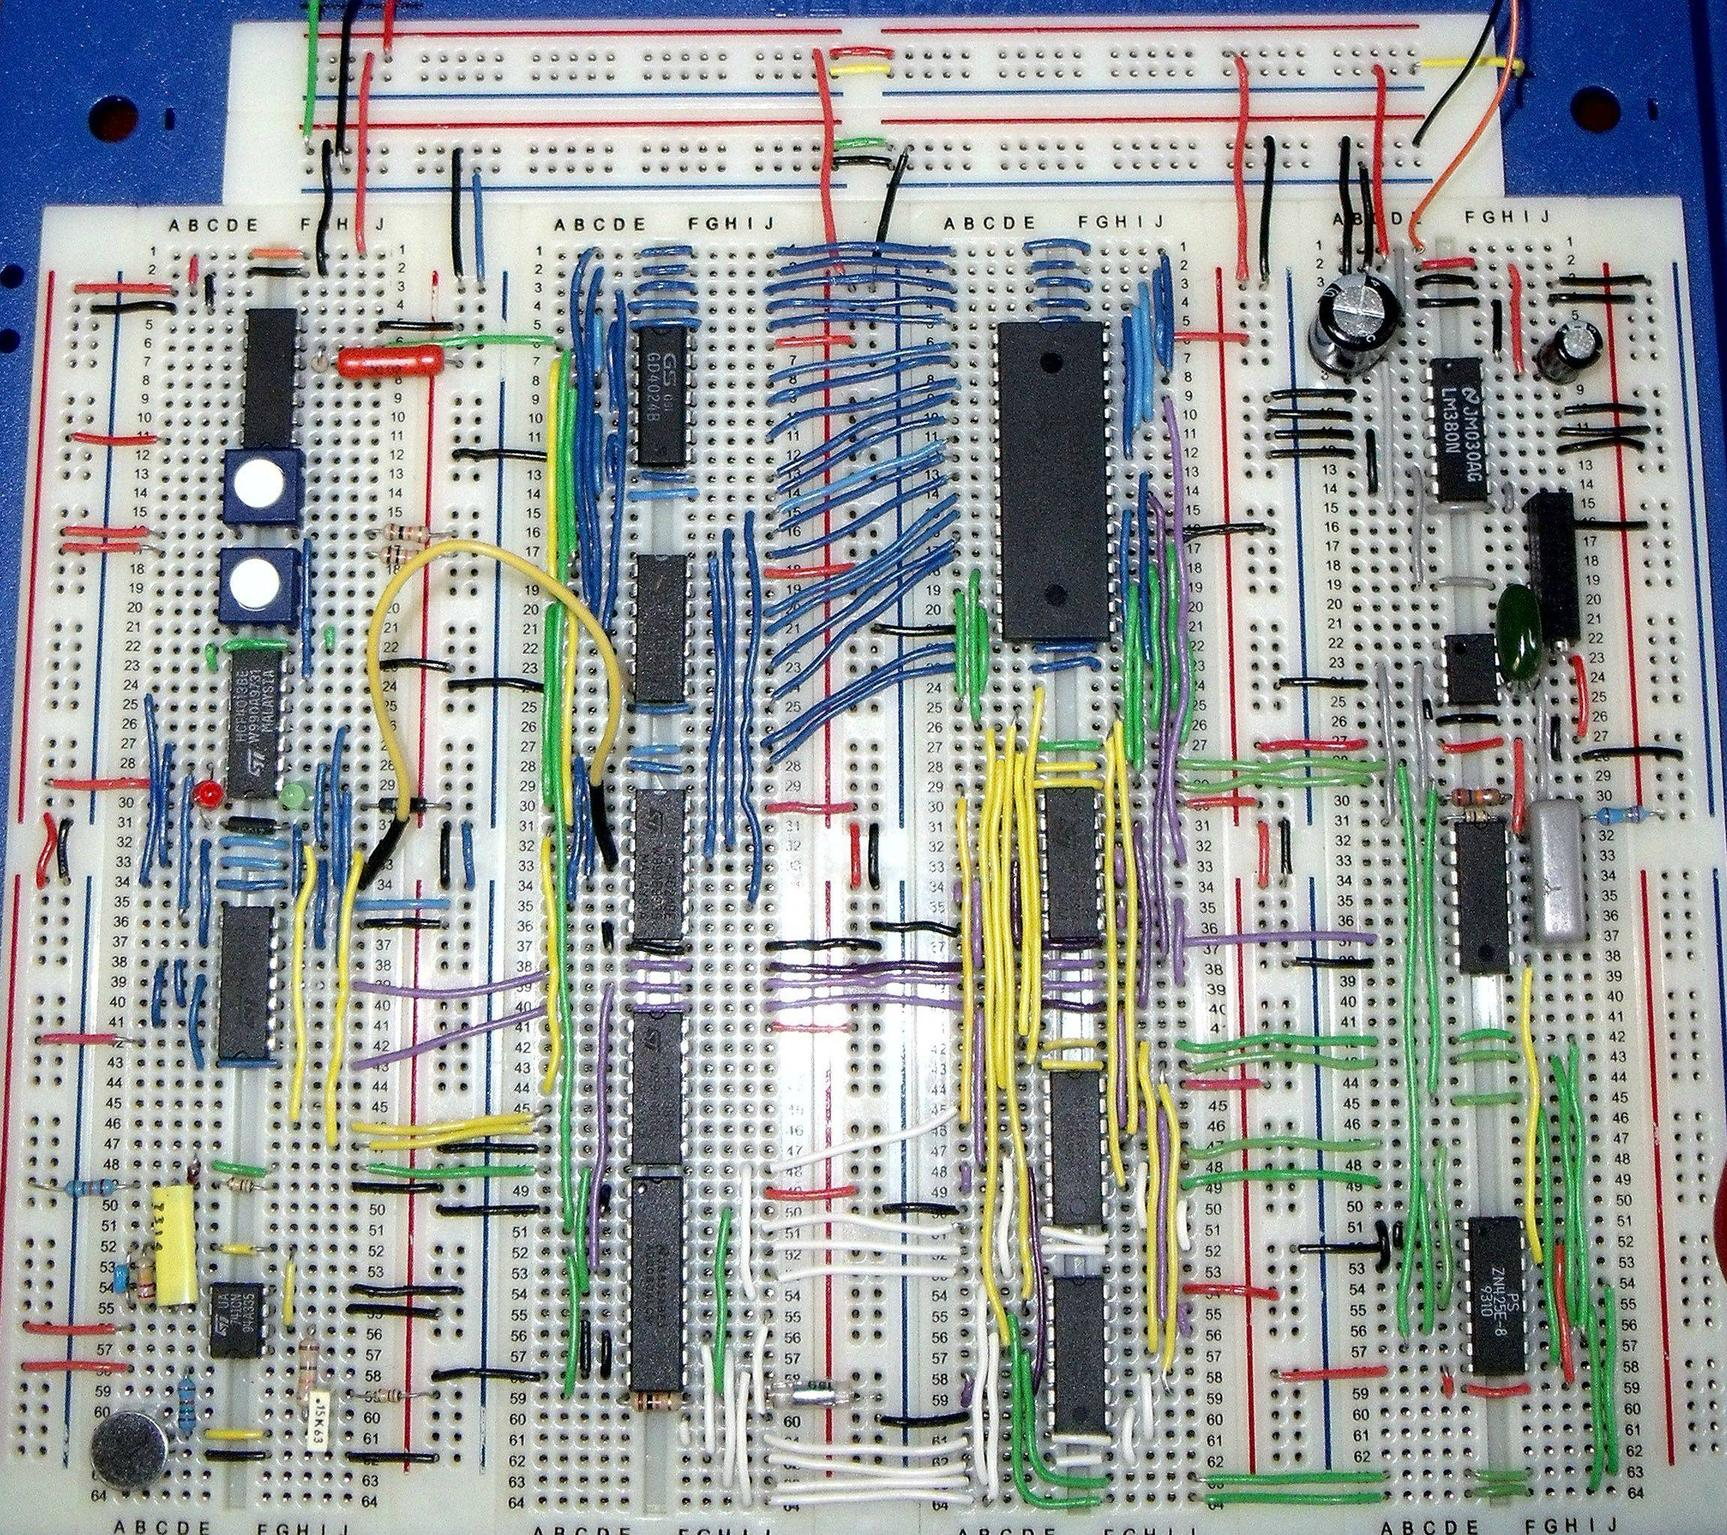
\includegraphics[width=1.0\textwidth]{breadboard.jpg} 
      \end{column}
    \end{columns}
  \end{frame}
  
  \begin{frame}
    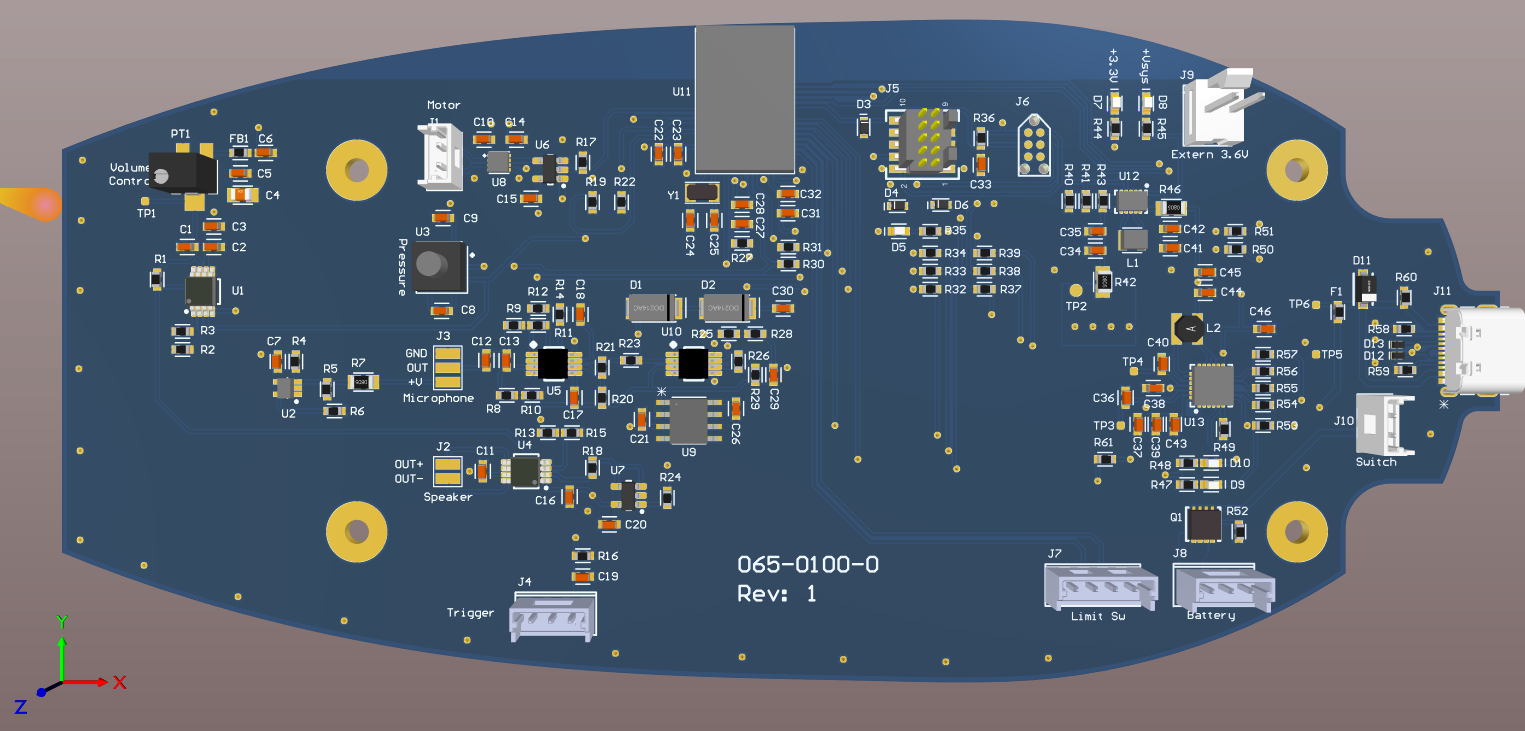
\includegraphics[width=1.0\textwidth]{pcb_rev1.png}
  \end{frame}
  
  \begin{frame}
    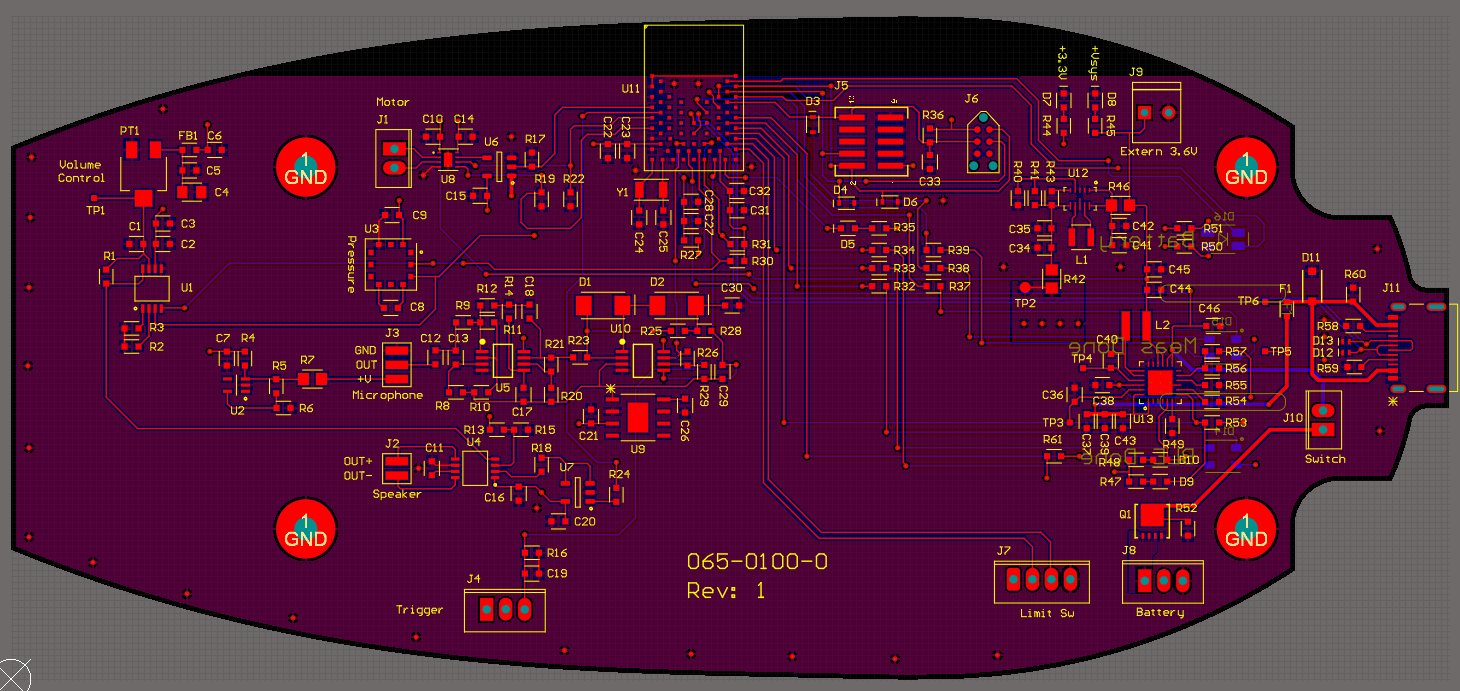
\includegraphics[width=1.0\textwidth]{pcb_layout_rev1.png}
  \end{frame}
  
  \begin{frame}
    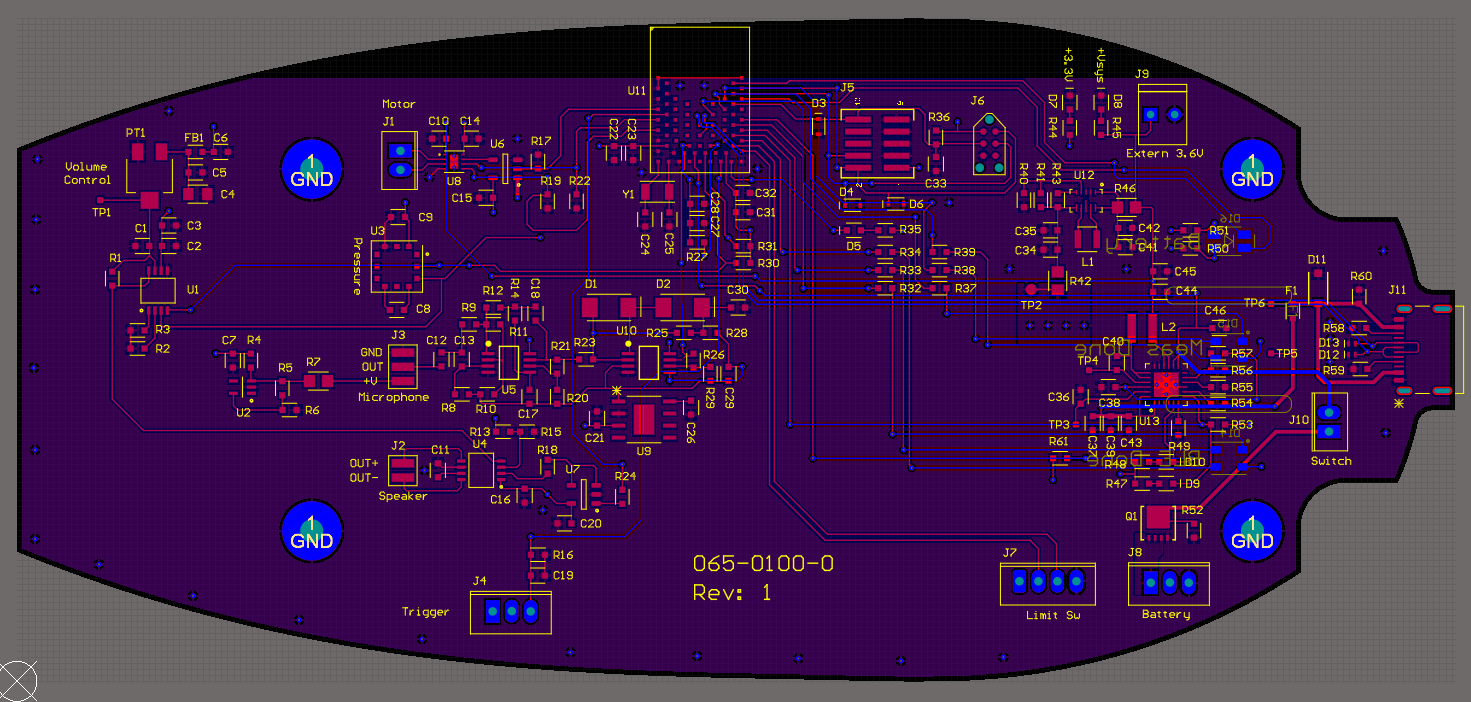
\includegraphics[width=1.0\textwidth]{pcb_layout_rev1_bottom.png}
  \end{frame}
  
  \begin{frame}
    \frametitle{Two-layer PCB}
  
    \begin{columns}
      \begin{column}{0.5\textwidth}
        \begin{itemize}
          \item Single-layer boards for ``trivial'' layouts.
          \item Two-layer board best balance of flexibility and complexity for ``simple'' layouts.
          \item $>$ 2 layers increases complexity (but putting power and ground on
          their own layers can be advantageous)
        \end{itemize}  
      \end{column}
      \begin{column}{0.5\textwidth}
        \centerline{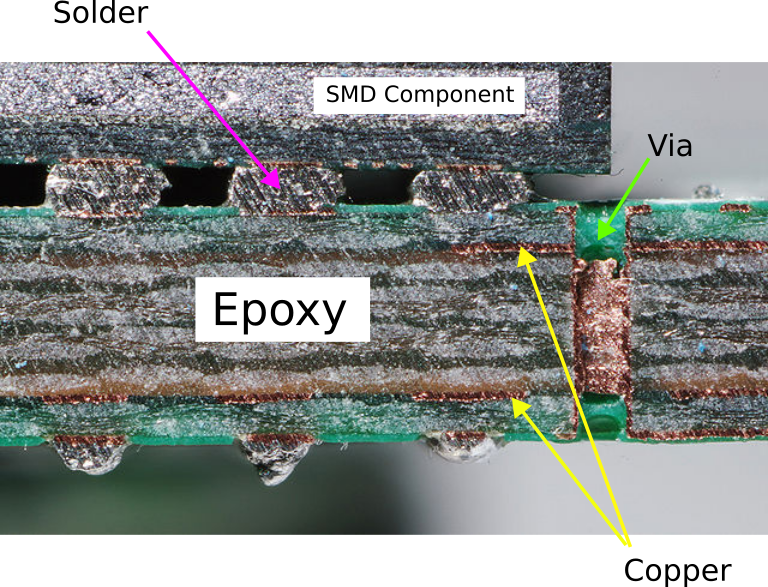
\includegraphics[width=1.0\textwidth]{pcb_layers_annotated.png}}
      \end{column}
    \end{columns}
  
  \end{frame}
  
  \begin{frame}
    \frametitle{THT vs. SMD}
    \begin{columns}
      \begin{column}{0.5\textwidth}
        \begin{itemize}
          \item Surface mount components on the same side as the traces
          \item Soldering using reflow.
          \item Thru-hole components on the opposite side from the traces (ease of
          soldering).
        \end{itemize}
      \end{column}
      \begin{column}{0.5\textwidth}
        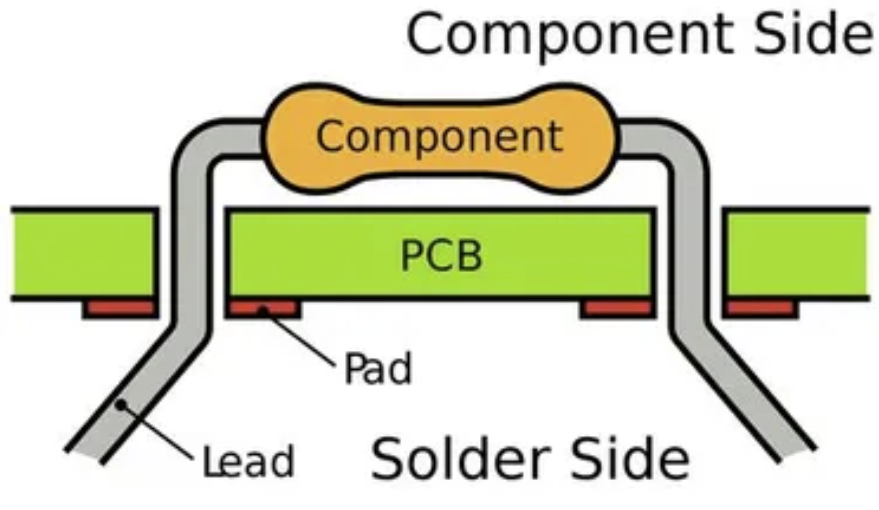
\includegraphics[width=0.75\textwidth]{tht_component.png}\\
        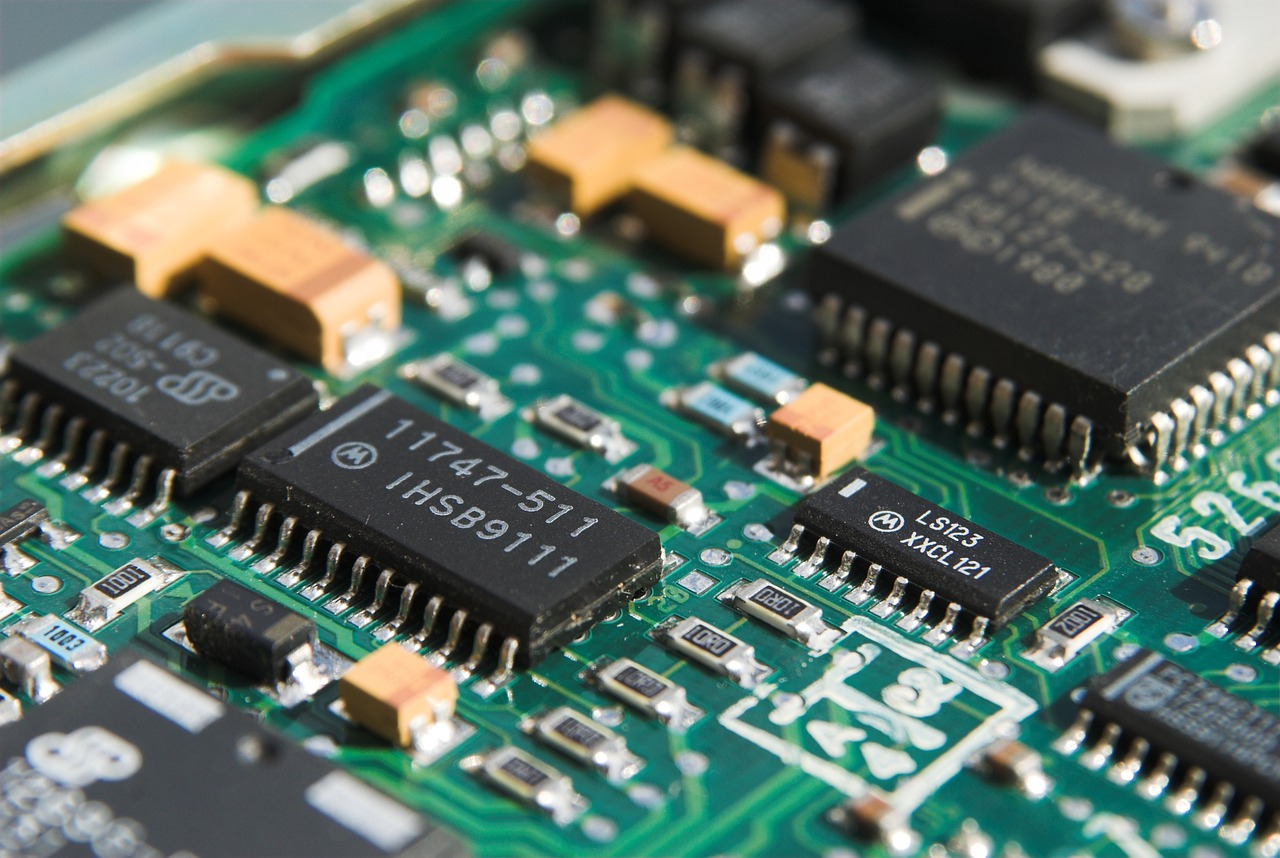
\includegraphics[width=0.65\textwidth]{smd_components.jpg}
      \end{column}
    \end{columns}
  \end{frame}
  
  \section{Workflow}
  
  \begin{frame}
    \frametitle{PCB Editor}
    \centerline{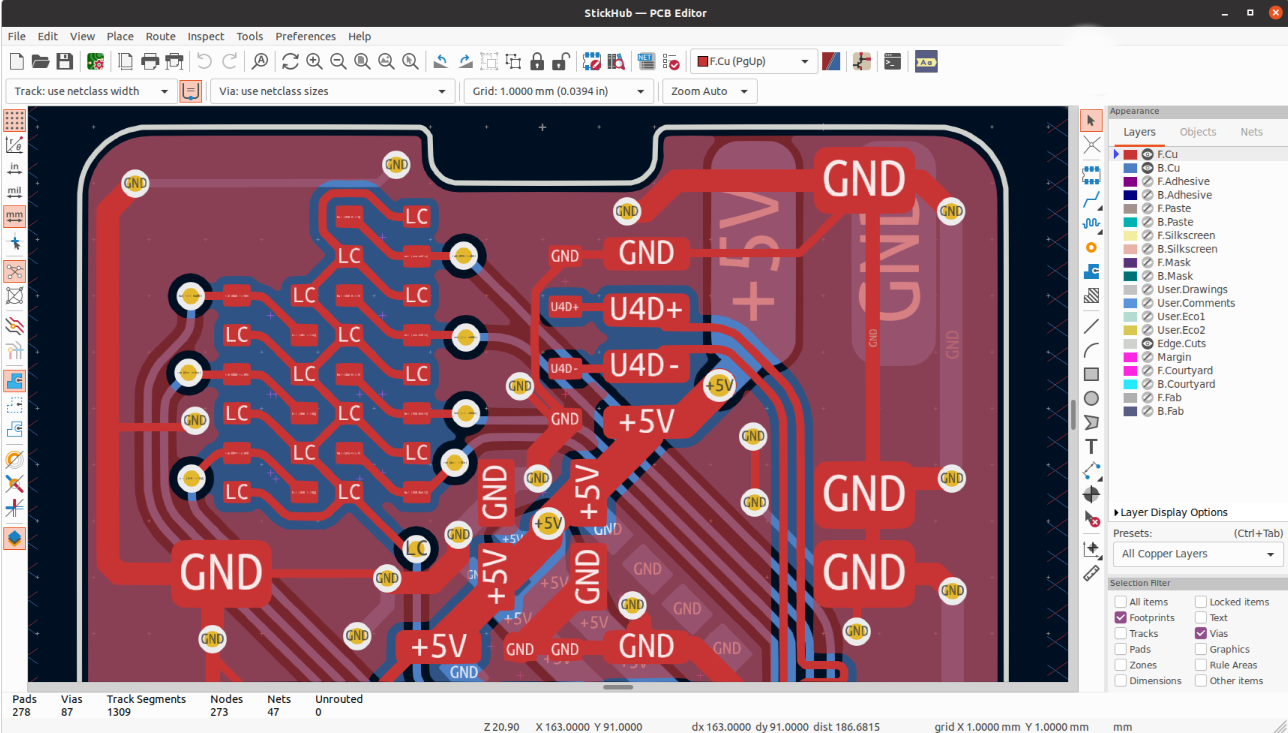
\includegraphics[width=0.8\textwidth]{pcbnew_ui.png}}
  \end{frame}
  
  \frame{
    \frametitle{Laying out a PCB}
    \begin{enumerate}
      \item Make sure that all parts are \textbf{annotated} and have \textbf{footprints}.
      \item Create PCB from schematic
      \item All component pins/pads that need to be connected with traces will be connected with airwires.
      \item Use \texttt{Graphics Lines} tool to create board outline (Layer:
      \texttt{Edge.Cuts})
      \item Layout components based on your design needs / constraints,
      considering orientation, board side, etc.
      \item Setup \textbf{Design Rules} (\texttt{File $\rightarrow$ Board Setup...}):
      \begin{itemize}
          \item Trace width ($\geq$ 20 mil)
          \item Drill diameter ($\geq$ 1 mm)
          \item Clearance ($\geq$ 32 mil)
      \end{itemize}
      \item Setup \textbf{Net Classes} for signal and power/ground (wider / more clearance).
    \end{enumerate}
  }
  
  \begin{frame}
    \frametitle{Laying out a PCB}
    \begin{enumerate}
      \setcounter{enumi}{7}
      \item Route traces
      \begin{itemize}
        \item Make sure that you are on the correct layer! 
      \end{itemize}
      \item Use \texttt{Filled Zone} tool to create a copper pour
      (\texttt{F/B.Cu}), usually associated with the \texttt{GND} net.
      \item Clearout other zones, as needed.
      \item Perform \textbf{Design Rule Check (DRC)}
    \end{enumerate}
  \end{frame}
  
  
  \section{Power / Ground}
  
  \begin{frame}
    \frametitle{Power Traces / Layers}
  
    \begin{columns}
      \begin{column}{0.5\textwidth}
        \begin{itemize}
          \item Larger trace width for greater power delivery (less resistance for
          more current).
          \item Even better to dedicate an entire layer
          \begin{itemize}
            \item More direct return paths
            \item Shielding (EMI)
            \item Reduce noise (switching)
            \item Dissipate heat
          \end{itemize}
        \end{itemize}
      \end{column}
        \begin{column}{0.5\textwidth}
          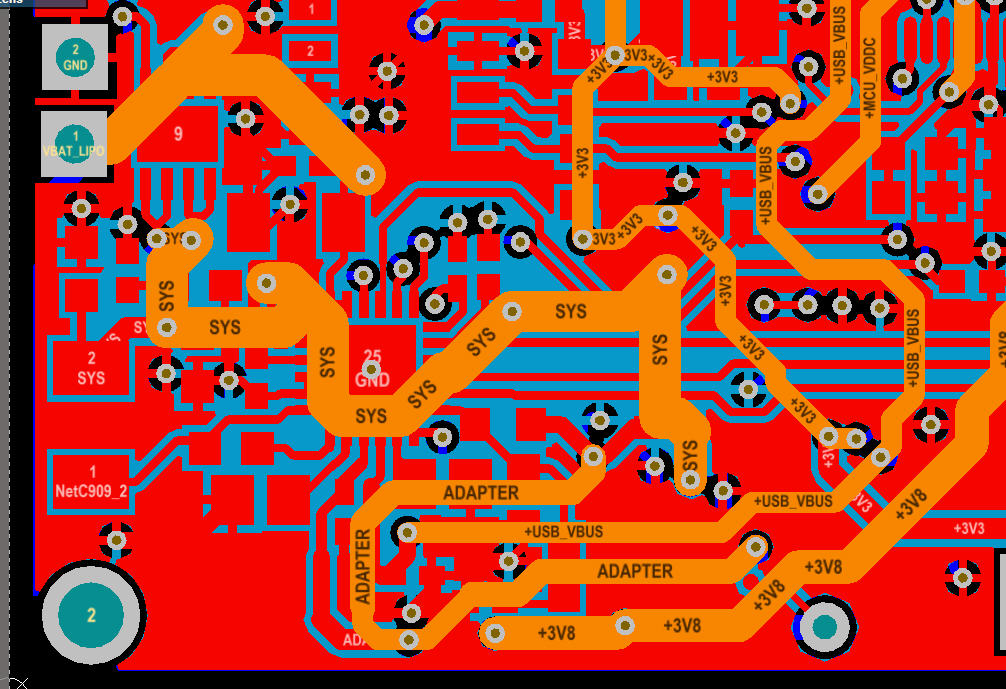
\includegraphics[width=1.0\textwidth]{pwr_vs_signal_traces.jpg}
        \end{column}
    \end{columns}
  
  \end{frame}
  
  \frame{
    \frametitle{Copper Ground Pours}
    \begin{columns}
      \begin{column}{0.5\textwidth}
      \begin{itemize}
        \item Help reject noise \& interference
        \item Lower impedance to ground
        \item Save milling time and bits!!
        \item Use jumper wire connections to electrically connect \texttt{GND} ``islands''.
      \end{itemize}
      \end{column}
        \begin{column}{0.5\textwidth}
          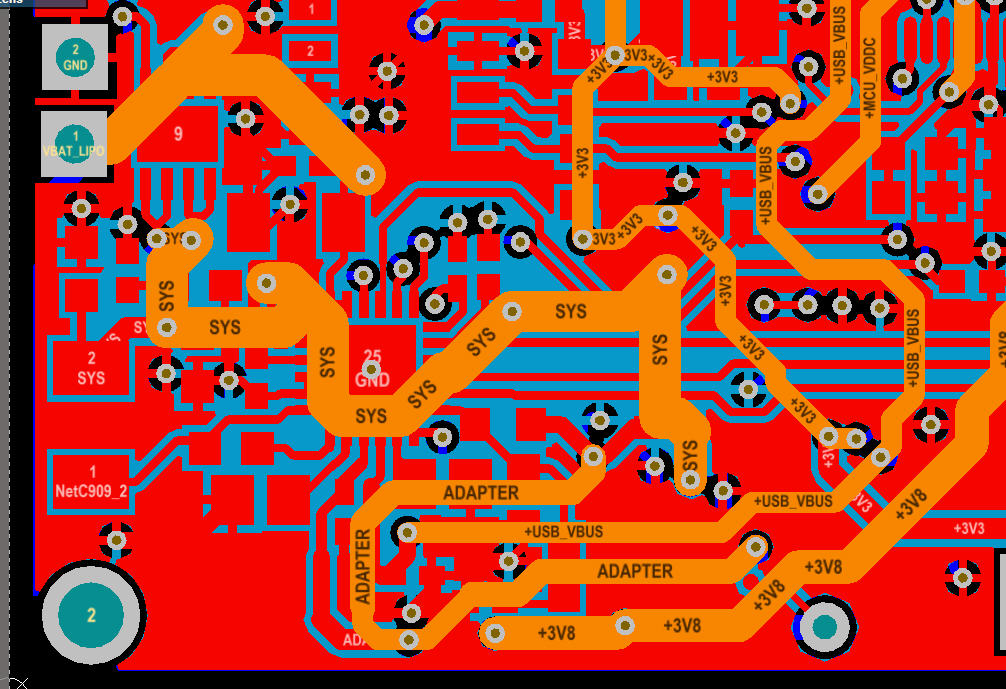
\includegraphics[width=1.0\textwidth]{pwr_vs_signal_traces.jpg}
        \end{column}
    \end{columns}
  }
  
  \begin{frame}
    \frametitle{Reducing Noise}
    \begin{itemize}
      \item Separate analog (\texttt{AGND}) and digital grounds (\texttt{GND}),
      and electrically connect using a \textbf{Net Tie}.
      \item Reduce trace ``loops'' (RF interference)
      \item Place decoupling capacitors next to power pins they are supporting.
    \end{itemize}
  \end{frame}
  
  \begin{frame}
      \frametitle{Thermal Relief}
  
      \centerline{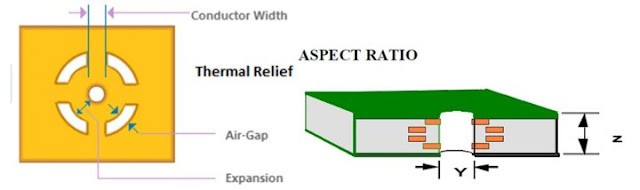
\includegraphics[width=0.75\textwidth]{thermal_relief.jpg}}
  
  \end{frame}
  
  
  \section{Tips}
  
  \frame{
    \frametitle{Kinds of Grounds}
  
    \begin{columns}
    \begin{column}{0.5\textwidth}
      \centerline{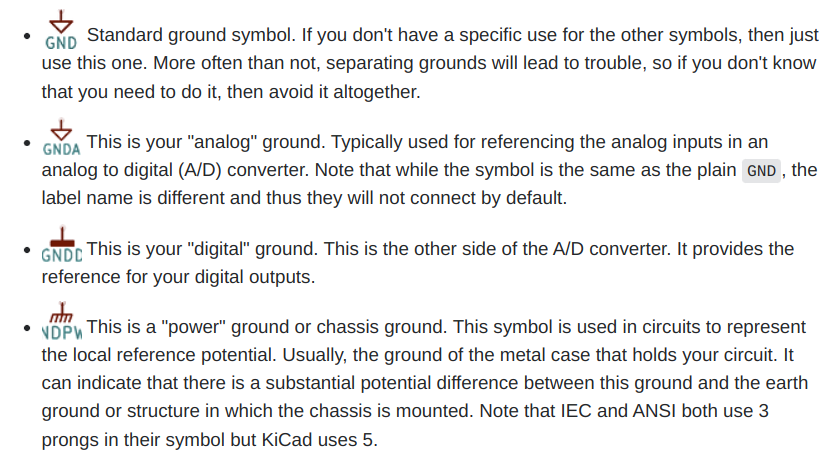
\includegraphics[width=1.0\textwidth]{grounds01.png}}
    \end{column}
    \begin{column}{0.5\textwidth}
      \centerline{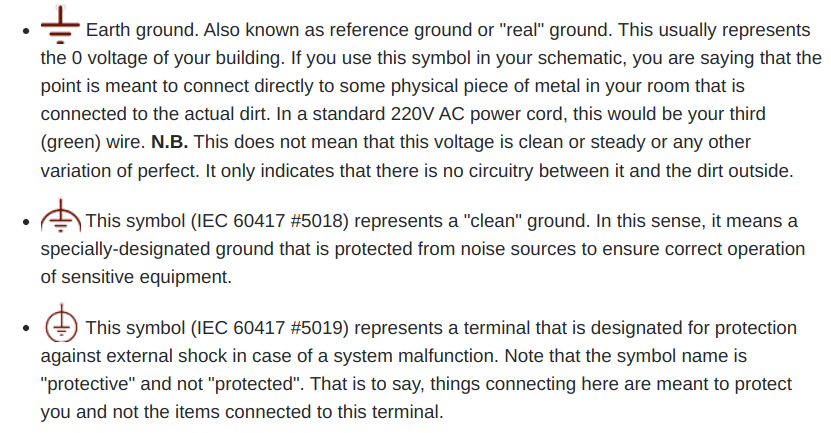
\includegraphics[width=1.0\textwidth]{grounds02.png}}
    \end{column}
  \end{columns}
  
  \begin{tiny}
  \url{https://electronics.stackexchange.com/questions/392911/kicad-5-what-is-the-significance-of-the-various-gnd-symbols}
  \end{tiny}
  }
  
  \frame{
    \frametitle{Tips-n-Tricks}
    \begin{itemize}
        \item You need to make sure that you update your PCB everytime you edit
        your schematic.  Failing to do so will create asyncrony of the two
        documents, which will be \emph{painful} to resolve.
       \item Clean up airwires with the \texttt{Ratsnest} tool.
       \item \textbf{Vias}: connections between top and bottom layers of a board.
       These can be plated or connected with a physical wire.
       \item Use jumpers for wire connections.
       \item Strategically place test pins / pads.
       \item Define ``clearout'' zones for areas where components cannot be placed
       (e.g., RF antenna)
       \item $\pm$ connections can be routed as a \textbf{Differential Pair}.
      \end{itemize}
  }
  
  \begin{frame}
    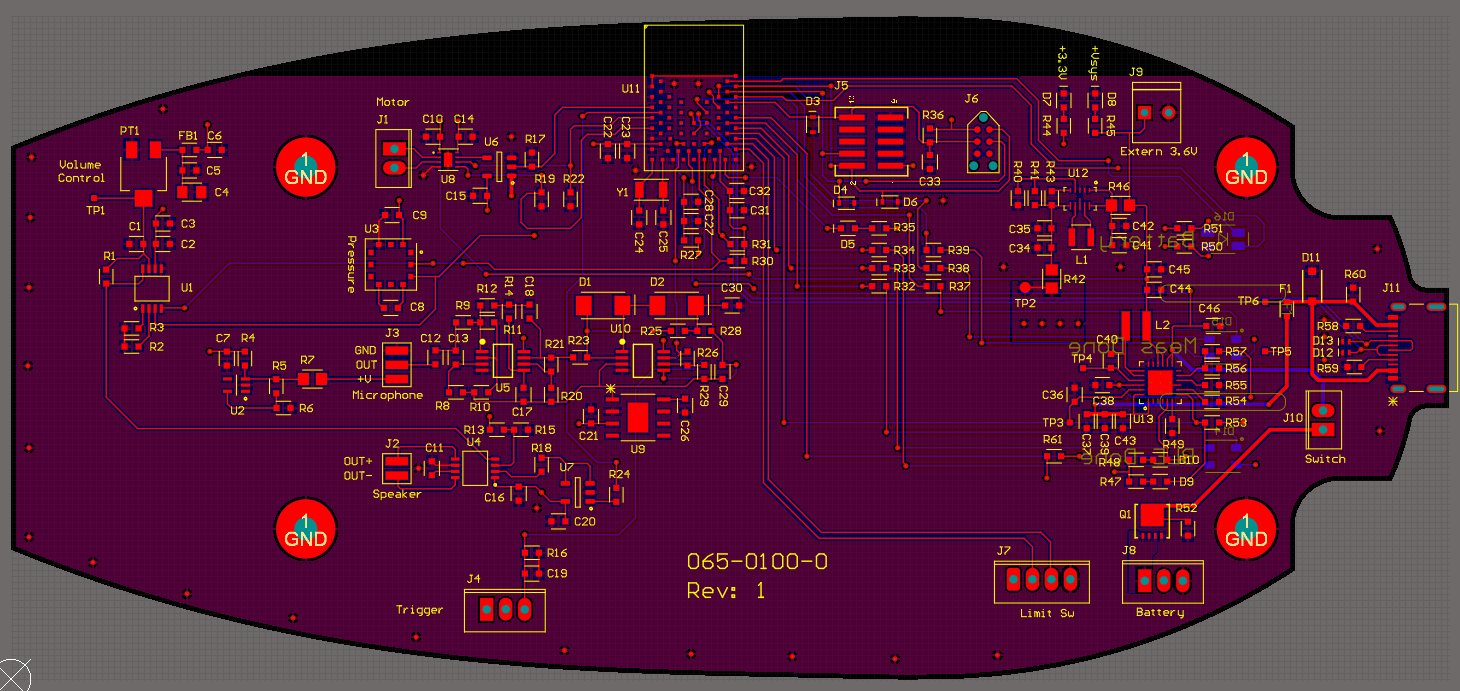
\includegraphics[width=1.0\textwidth]{pcb_layout_rev1.png}
  \end{frame}
  
  \begin{frame}
    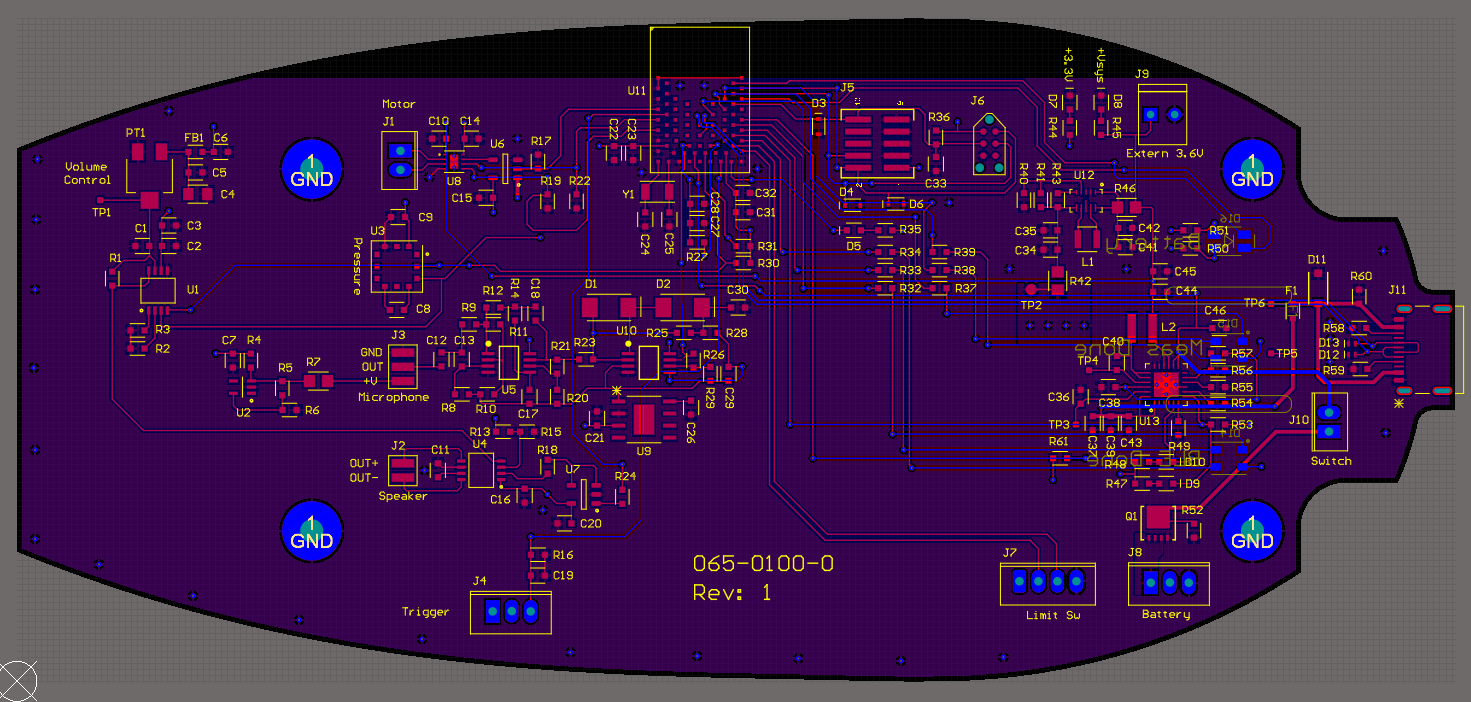
\includegraphics[width=1.0\textwidth]{pcb_layout_rev1_bottom.png}
  \end{frame}
  
  \begin{frame}
    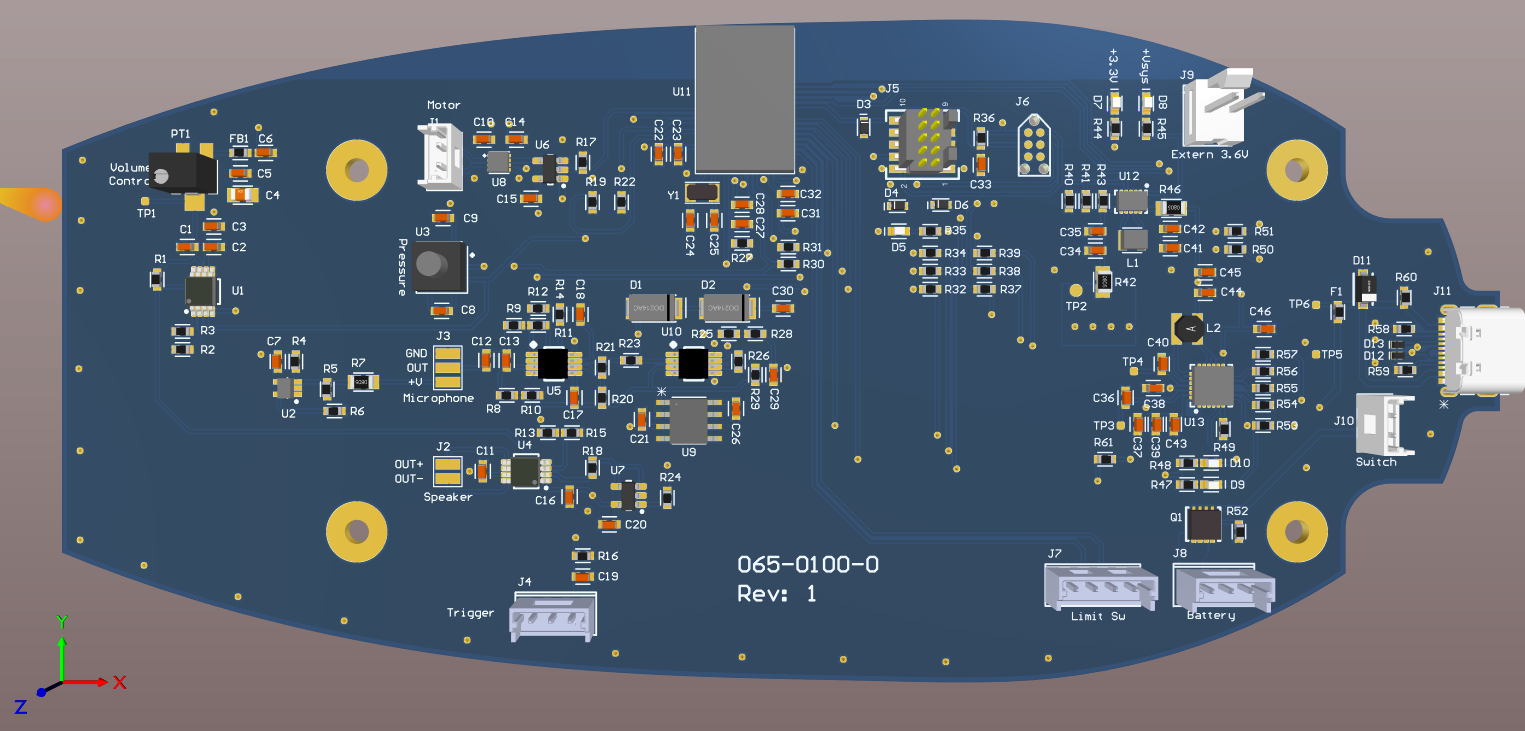
\includegraphics[width=1.0\textwidth]{pcb_rev1.png}
  \end{frame}
  
\section{Resources}

\begin{frame}
\frametitle{Resources}
\begin{itemize}
    \item \href{https://learn.sparkfun.com/tutorials/pcb-basics}{PCB Basics (SparkFun)}
    \item \href{https://mlp6.pages.oit.duke.edu/Medical-Electrical-Equipment/How\_to\_Design\_the\_Perfect\_PCB.pdf}{How to Design the Perfect PCB}
    \item \href{https://docs.kicad.org/6.0/en/pcbnew/pcbnew.html}{KiCad Docs: PCB Editor}
    \item \href{https://gitlab.oit.duke.edu/mlp6/kicad_test}{Example KiCad Project}
    \item \href{https://resources.pcb.cadence.com/blog/2020-grounding-and-voltage-routing-considerations-in-pcb-design-e2ek}{Grounding and Voltage Routing Considerations in PCB Design}
    \item \href{https://resources.pcb.cadence.com/blog/2021-effective-pcb-trace-width-and-spacing}{Effective PCB Trace Width and Spacing}
\end{itemize}
\end{frame}

\end{document}
